\documentclass{article}
% generated by Madoko, version 1.0.0-rc5
%mdk-data-line={1}


\usepackage[heading-base={2},section-num={False},bib-label={True}]{madoko2}


\begin{document}



%mdk-data-line={5}
\mdxtitleblockstart{}
%mdk-data-line={5}
\mdxtitle{\mdline{5}Optimization of the DNN program on the CPU+MIC Platform}%mdk
\mdxauthorstart{}
%mdk-data-line={10}
\mdxauthorname{\mdline{10}University of Electronic Secience and Technology of China}%mdk
\mdxauthorend\mdtitleauthorrunning{}{}\mdxtitleblockend%mdk

%mdk-data-line={6}
\section{\mdline{6}1.\hspace*{0.5em}\mdline{6}Preface}\label{sec-preface}%mdk%mdk

%mdk-data-line={7}
\noindent\mdline{7}In the section we are required to optimize a \mdline{7}\mdcode{DNN(deep~neural~network)}\mdline{7}
program based on a standalone hybrid CPU+MIC platform. The detailed
configuration is as follows:%mdk

%mdk-data-line={11}
\mdline{11}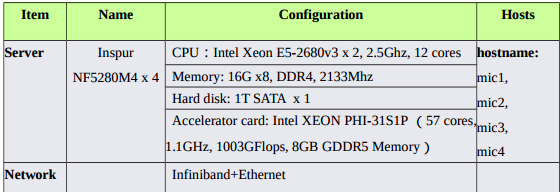
\includegraphics[keepaspectratio=true,width=\dimmin{}{\dimwidth{0.90}}]{images/2016-02-18-23-01-13-}{}\mdline{11}%mdk

%mdk-data-line={15}
\noindent\mdline{15}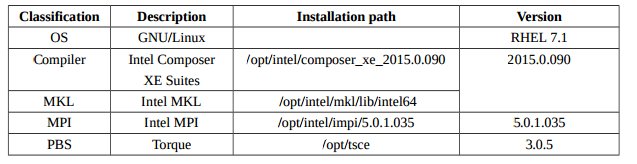
\includegraphics[keepaspectratio=true,width=\dimmin{}{\dimwidth{0.90}}]{images/2016-02-18-23-13-11-}{}\mdline{15}%mdk

%mdk-data-line={21}
\section{\mdline{21}2.\hspace*{0.5em}\mdline{21}Analysis of the serial program}\label{sec-analysis-of-the-serial-program}%mdk%mdk

%mdk-data-line={22}
\noindent\mdline{22}First, we generate a call graph by using \mdline{22}\textbf{Google perfools}\mdline{22},
 a open source performance profiler, to have a glance though it. Every
 square represents a function, and the bigger square is, the more time
 corresponding function cost.
Obviously, the hot spot is something about \mdline{26}\textbf{MKL}\mdline{26}. After googling
and searching Intel document we know that MKL provides BLAS routinues,
which includes a serial funcition named \mdline{28}\textquotedblleft{}cblas\_?gemm\textquotedblright{}\mdline{28}
to compute a matrix-matrix product with general matrices.%mdk%mdk


\end{document}
